%!TEX program = xelatex
\documentclass[a4paper,UTF8]{ctexart}
\usepackage[unicode=true,colorlinks,linkcolor=blue,urlcolor=blue,bookmarksnumbered=true]{hyperref}
\usepackage{latexsym,amssymb,amsmath,amsbsy,amsopn,amstext,amsthm,amsxtra,color,multicol,bm,calc,ifpdf}
\usepackage{graphicx}
\usepackage{diagbox}   % 绘制表格斜线
\usepackage{enumerate}
\usepackage{epstopdf}
\usepackage{fancyhdr}
\usepackage{subfigure}
\usepackage{listings}
\usepackage{multirow}
\usepackage{makeidx}
\usepackage{xcolor} 
\usepackage{tikz}
\usepackage{fontspec}                            % 建立索引宏包
\graphicspath{{figures/}}  % 设置图片搜索路径
\theoremstyle{plain} \newtheorem{theorem}{定理}[section]
\theoremstyle{plain} \newtheorem{definition}{定义}[section]
\theoremstyle{plain} \newtheorem{lemma}{引理}[section]
\theoremstyle{plain} \newtheorem{proposition}{命题}[section]
\theoremstyle{plain} \newtheorem{example}{例}[section]
\theoremstyle{plain} \newtheorem{remark}{注}[section]
\theoremstyle{plain} \newtheorem{corollary}{推论}[section]
\newfontfamily\courier{Courier New}
\lstset{linewidth=1.1\textwidth,
        numbers=left, %设置行号位置 
        basicstyle=\small\courier,
        numberstyle=\tiny\courier, %设置行号大小  
        keywordstyle=\color{blue}\courier, %设置关键字颜色  
        %identifierstyle=\bf,
        commentstyle=\it\color[cmyk]{1,0,1,0}\courier, %设置注释颜色 
        stringstyle=\it\color[RGB]{128,0,0}\courier,
        %framexleftmargin=10mm,
        frame=single, %设置边框格式  
        backgroundcolor=\color[RGB]{245,245,244},
        %escapeinside=``, %逃逸字符(1左面的键),用于显示中文  
        breaklines, %自动折行  
        extendedchars=false, %解决代码跨页时,章节标题,页眉等汉字不显示的问题  
        xleftmargin=2em,xrightmargin=2em, aboveskip=1em, %设置边距  
        tabsize=4, %设置tab空格数  
        showspaces=false %不显示空格  
        basicstyle=\small\courier
       }  
\newenvironment{mysolution}{{\color{blue} 解}: }{{\color{magenta}\qed}}
\newcommand\diff{\,{\mathrm d}} %定义微分d
\newcommand{\p}[3]{\frac{\partial^{#1}#2}{\partial{#3}^{#1}}}  %定义求偏导算子
\newcommand{\ucite}[1]{\textsuperscript{\cite{#1}}}  %参考文献引用:上标用\ucite{ },文中用\cite{ }
\def\layersep{2.5cm}

\begin{document}
\title{

\includegraphics[width=0.65\textwidth]{onepiece.pdf}\\
\vspace{2em}
\textbf{神经网络学习笔记}}
\author{\emph{李向阳} \quad {\color{blue}d1142845997@gmail.com}
}
\date{}

\maketitle
\thispagestyle{empty}

\newpage


\tableofcontents

\newpage

\section{人工神经网络}
前面我们已经介绍了线性回归、Logistic 回归、Softmax 回归和 SVM 模型, 其中逻辑回归和 SVM 都是分类的重要方法, 不过我们主要介绍了二分类, 它们当然也可推广用于多分类问题, 不过要处理多分类问题, 我们有另外一个更好的办法, 那就是神经网络. 因此, 本篇章就先来简要介绍一下人工神经网络(Artifical Neural Network, 即 ANN).

当然, 引入神经网络并不单纯是处理多分类的问题, 它有还有很多引入的角度. 比如, 当变量特征数$n$非常多时, 利用神经网络就比较方便. 这尤其体现在图像处理领域, 为了给图像分类, 我们一般是把图像转化为一个灰度矩阵(比如$28 \times 28$),然后把所有的灰度值看成一个向量(维数为$784$), 任何一个图片都可以这样处理,  这样就可以利用机器学习的方法, 即相当于样本有$n = 784$个变量特征, 然后决定样本的类别. 一个简单而典型的例子便是手写数字识别.


\subsection{数据集}
必须先指出一点, 还是记号的问题. 这在前面已经提到过多次, 但在神经网络的模型里大多数文献的记号都更为复杂(与前面的回归模型、SVM 模型相比), 因此是一件头疼的事情, 我尽量按照通用的记号.

假设样本有$n$个特征, 记为$\bm{x} = (x_{1},x_{2},\cdots,x_{n})^{T}$,由于对应的类别可能有很多而不再只是两类, 比如说有$K$类, 因此现在得换一些方法(之前用$y = 0, 1$或$y = \pm 1$表示正负类). 一种方法是让$y$有$K$个取值, 用$y = k(k = 1, 2, \cdots, K)$表示属于第$k$类. 另一种方法是把类别表示为一个$K$维向量, 其第$k$个分量取$1$, 其余分量全为$0$表示样本属于第$k$类. 这里我们采用后一种方法, 即用向量$\bm{y} = (y_{1}, y_{2}, \cdots, y_{K})^{T}$表示, 其中分量$y_{k} = 1$, 其余为$0$表示样本属于第$k$类.

现在有$m$个样本, 即$\{ \bm{x}^{(i)}, \bm{y}^{(i)} \}, i = 1, 2, \cdots, m$, 其中
\begin{equation*}
\bm{x}^{(i)} = (x_{1}^{(i)}, x_{2}^{(i)}, \cdots, x_{n}^{(i)})^{T},i = 1, 2, \cdots, m
\end{equation*}


\subsection{神经元}
为了描述神经网络模型, 我们先从神经元(Neuron)说起.

单个的神经元和之前的 Logistic 回归模型是类似的, 即神经元接受输入$x_{1}, x_{2}, \cdots, x_{n}$, 然后输出该神经元的活性值$a$, 如下:
\begin{align*}
z & = \bm{w}^{T} \bm{x} + b \\ 
a & = f(z) = f(\bm{w}^{T} \bm{x} + b)
\end{align*}

其中$f(\cdot)$称为激活函数(activation function), 如果$f(\cdot)$取为 sigmoid 函数的话, 那就和 Logistic 回归很像了, 只不过那里我们把参数用$\bm{\theta}$表示而已(引入$\theta_0 = 1$). 这里我们分开用$\bm{w}$和$b$表示, 显然, $\bm{w}$表示各个特征的权重, 而$b$称为偏置(之前称$\theta_0$为常数), 有了单独的参数$b$, 我们就不必像 Logistic 回归那样引入$x_{0} = 1$了.
\begin{figure}[!htb]
  \centering
  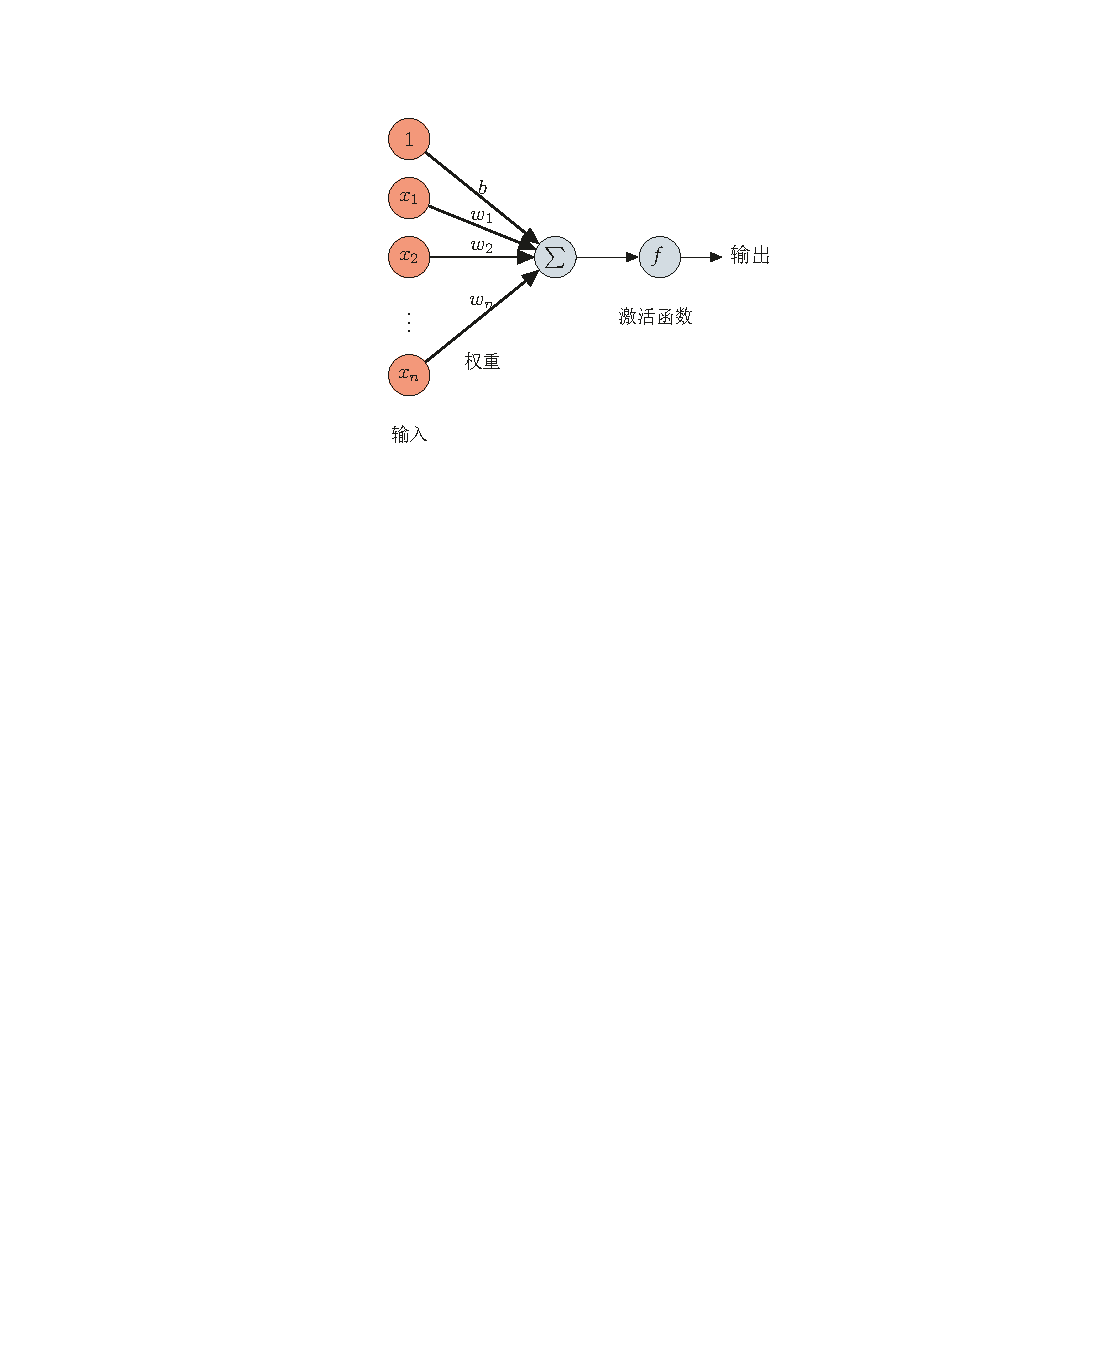
\includegraphics[width = 0.85 \textwidth]{neuron.pdf}
  \caption{神经元}
  \label{neuron}
\end{figure}


激活函数有很多种选择, 比如 sigmoid 函数、tanh 函数等等. 其中 tanh 函数是 sigmoid 函数的一种变体, 它的取值范围为$[-1,1]$, 而不是 sigmoid 函数的$[0,1]$. 在本文讨论中, 我们选用 sigmoid 函数
\begin{equation*}
f(z) = \frac{1}{1 + \mathrm{e}^{-z}}
\end{equation*}

\begin{figure}[!htb]
  \centering
  \subfigure[sigmoid 函数]{
  \label{sigmoid}
  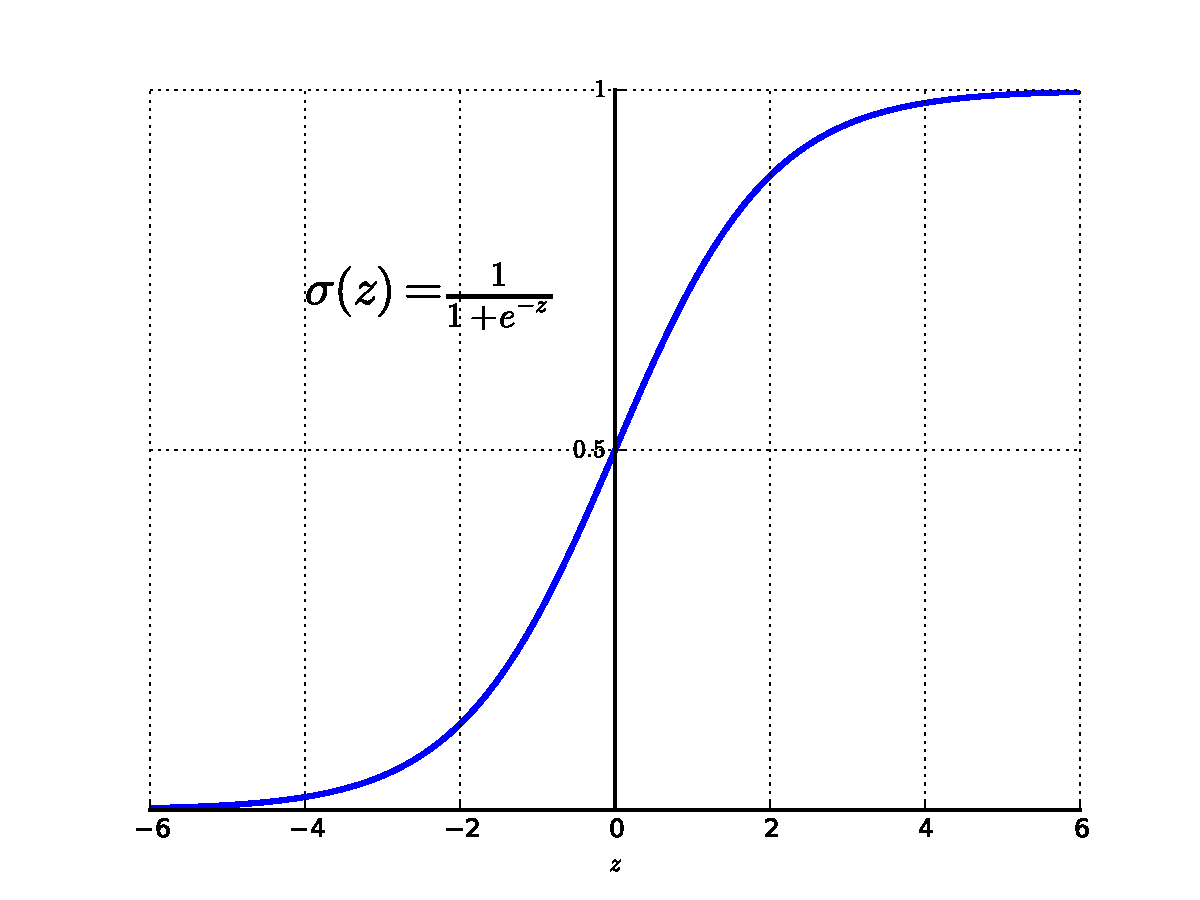
\includegraphics[width=1.9in]{sigmoid.pdf}
  }
  \hspace{0.2in}
  \subfigure[tanh 函数]{
  \label{tanh}
  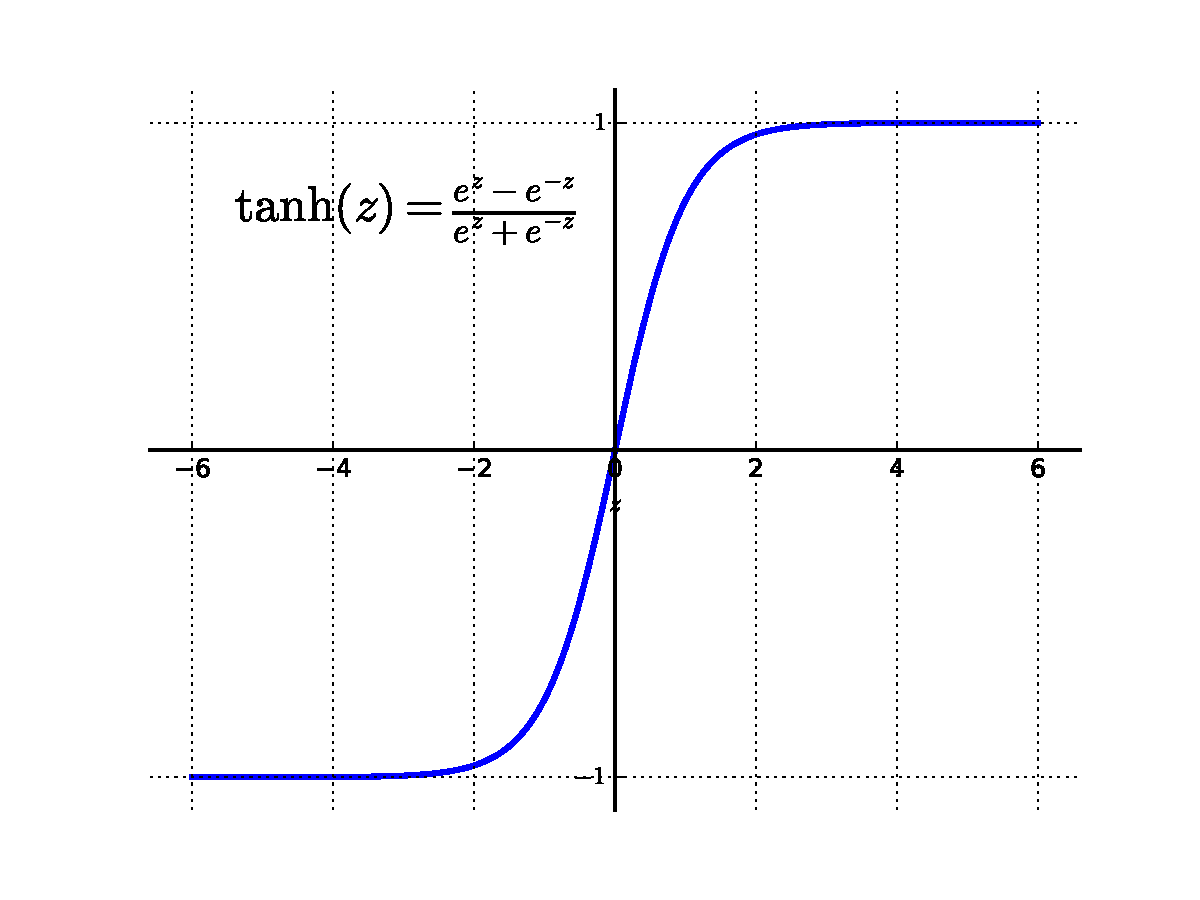
\includegraphics[width=1.9in]{tanh.pdf}
  }
  \caption{激活函数}
  \label{activate}
\end{figure}

有一个等式可能在推导时比较有用, 如果选择激活函数为 sigmoid 函数$f(z) = 1 / (1 + \mathrm{exp} (-z))$, 那么它的导数为$f'(z) = f(z) (1 - f(z))$, 这个根据定义验证即可(如果选择 tanh 函数, 那么则有$f'(z) = 1 - (f(z))^2$).

那么神经元输出的$a$有什么用呢?

在Logistic回归中, 我们是根据$a$的大小来将样本分为$2$类, 如果$a > 0.5$则归为正类, 否则归为负类. 在神经网络模型中, 有许许多多的这样的神经元, 其实每一个神经元输出的$a$值是当成一个新的特征的值来作为下一个神经元的输入的, 如下图\ref{neuralnet}所示.
\begin{figure}[!htb]
  \centering
  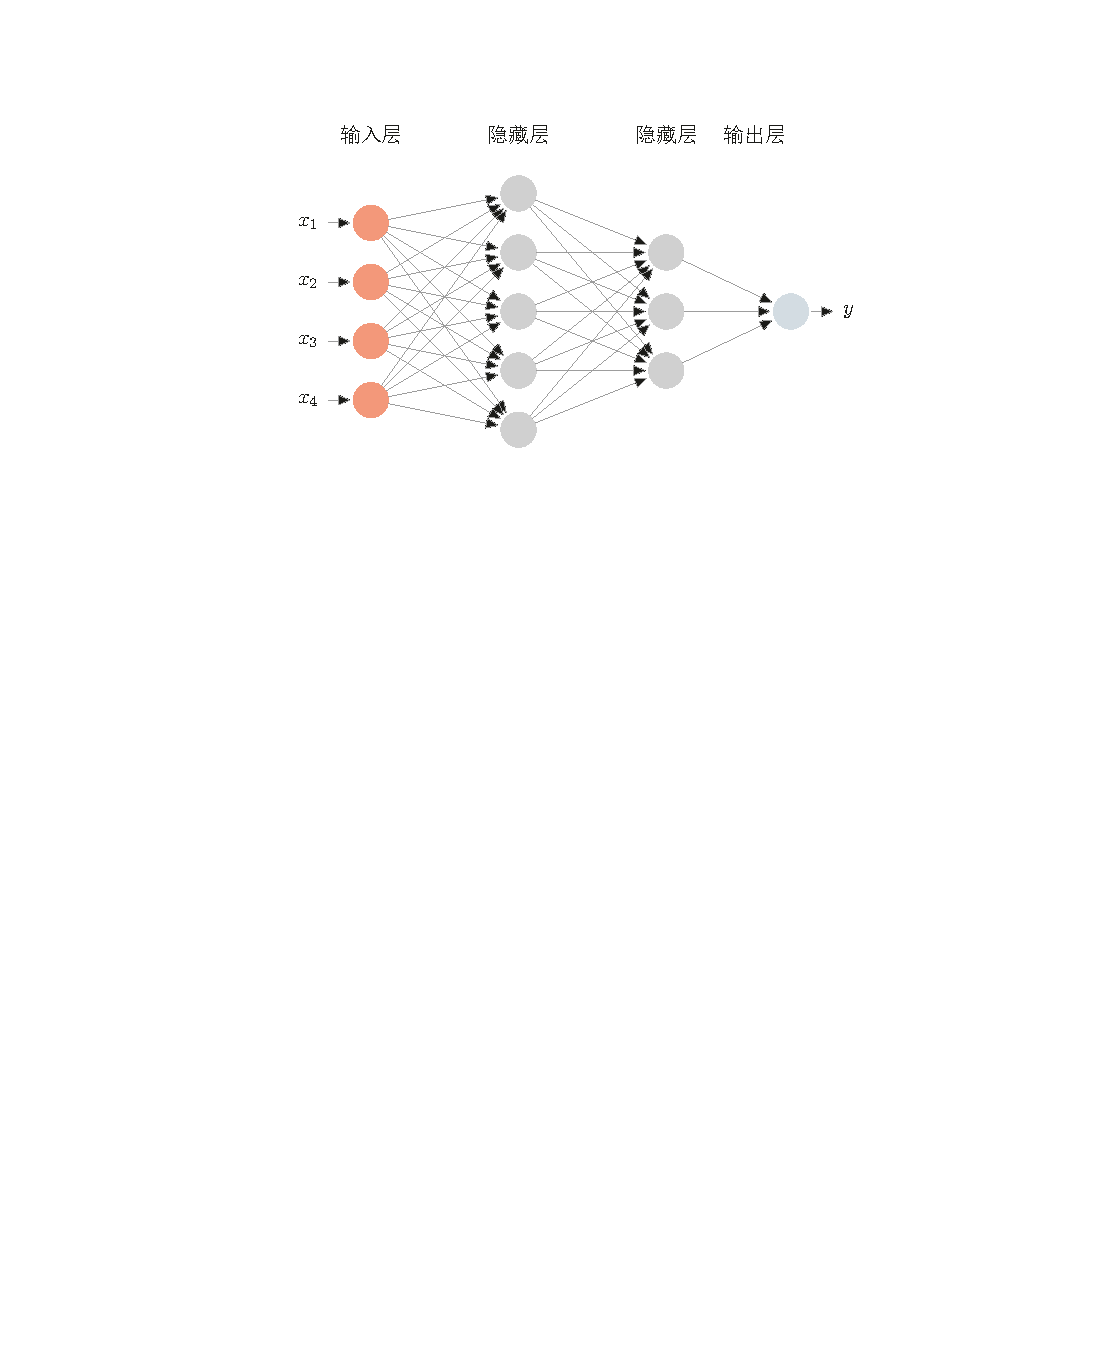
\includegraphics[width = 0.80 \textwidth]{neuralnetwork.pdf}
  \caption{神经网络示意图}
  \label{neuralnet}
\end{figure}


\begin{figure}[!htb]
\centering
\begin{tikzpicture}[shorten >=1pt,->,draw=black!50, node distance=\layersep]
    \tikzstyle{every pin edge}=[<-,shorten <=1pt]
    \tikzstyle{neuron}=[circle,fill=black!25,minimum size=17pt,inner sep=0pt]
    \tikzstyle{input neuron}=[neuron, fill=green!50];
    \tikzstyle{output neuron}=[neuron, fill=red!50];
    \tikzstyle{hidden neuron}=[neuron, fill=blue!50];
    \tikzstyle{annot} = [text width=4em, text centered]

    % Draw the input layer nodes
    \foreach \name / \y in {1,...,4}
    % This is the same as writing \foreach \name / \y in {1/1,2/2,3/3,4/4}
        \node[input neuron, pin=left:$x_{\y}$] (I-\name) at (0,-\y) {};

    % Draw the hidden layer nodes
    \foreach \name / \y in {1,...,5}
        \path[yshift=0.5cm]
            node[hidden neuron] (H-\name) at (\layersep,-\y cm) {};

    % Draw the output layer node
    \node[output neuron,pin={[pin edge={->}]right:$\bm{y}$}, right of=H-3] (O) {};

    % Connect every node in the input layer with every node in the
    % hidden layer.
    \foreach \source in {1,...,4}
        \foreach \dest in {1,...,5}
            \path (I-\source) edge (H-\dest);

    % Connect every node in the hidden layer with the output layer
    \foreach \source in {1,...,5}
        \path (H-\source) edge (O);

    % Annotate the layers
    \node[annot,above of=H-1, node distance=1cm] (hl) {隐藏层};
    \node[annot,left of=hl] {输入层};
    \node[annot,right of=hl] {输出层};
\end{tikzpicture}
\end{figure}


\tikzset{%
  every neuron/.style={
    circle,
    draw,
    minimum size=1cm
  },
  neuron missing/.style={
    draw=none, 
    scale=4,
    text height=0.333cm,
    execute at begin node=\color{black}$\vdots$
  },
}

\begin{figure}[!htb]
\centering
\begin{tikzpicture}[x=1.5cm, y=1.5cm, >=stealth]

\foreach \m/\l [count=\y] in {1,2,3,missing,4}
  \node [every neuron/.try, neuron \m/.try] (input-\m) at (0,2.5-\y) {};

\foreach \m [count=\y] in {1,missing,2}
  \node [every neuron/.try, neuron \m/.try ] (hidden-\m) at (2,2-\y*1.25) {};

\foreach \m [count=\y] in {1,missing,2}
  \node [every neuron/.try, neuron \m/.try ] (output-\m) at (4,1.5-\y) {};

\foreach \l [count=\i] in {1,2,3,n}
  \draw [<-] (input-\i) -- ++(-1,0)
    node [above, midway] {$x_\l$};

% \foreach \l [count=\i] in {1,n}
%   \node [above] at (hidden-\i.north) {$H_\l$};

% \foreach \l [count=\i] in {1,n}
%   \draw [->] (output-\i) -- ++(1,0)
%     node [above, midway] {$O_\l$};

\foreach \i in {1,...,4}
  \foreach \j in {1,...,2}
    \draw [->] (input-\i) -- (hidden-\j);

\foreach \i in {1,...,2}
  \foreach \j in {1,...,2}
    \draw [->] (hidden-\i) -- (output-\j);

\foreach \l [count=\x from 0] in {输入, 隐藏, 输出}
  \node [align=center, above] at (\x*2,2) {\l  层};

\end{tikzpicture}
\end{figure}




\subsection{前向神经网络模型}
有了神经元, 我们可以以神经元为节点来构建一个网络. 不同的神经网络模型有着不同网络连接的拓扑结构. 一种比较直接的拓扑结构是前向网络. 前向神经网络(Feed-forward Neural Network)是最早发明的简单人工神经网络. 各神经元分别属于不同的层, 每一层的神经元可以接收前一层神经元的信号, 并产生信号输出到下一层. 第一层叫输入层, 最后一层叫输出层, 其它中间层叫做隐藏层. 整个网络中无反馈, 信号从输入层向输出层单向传播, 可用一个有向无环图表示. 上图\ref{neuralnet}中就是一个前向神经网络的示例.

接下来引入一些概念和(复杂)的记号, 为了方便说明, 我们把偏置项也画出来, 可见下图\ref{notation}.
\begin{figure}[!htb]
  \centering
  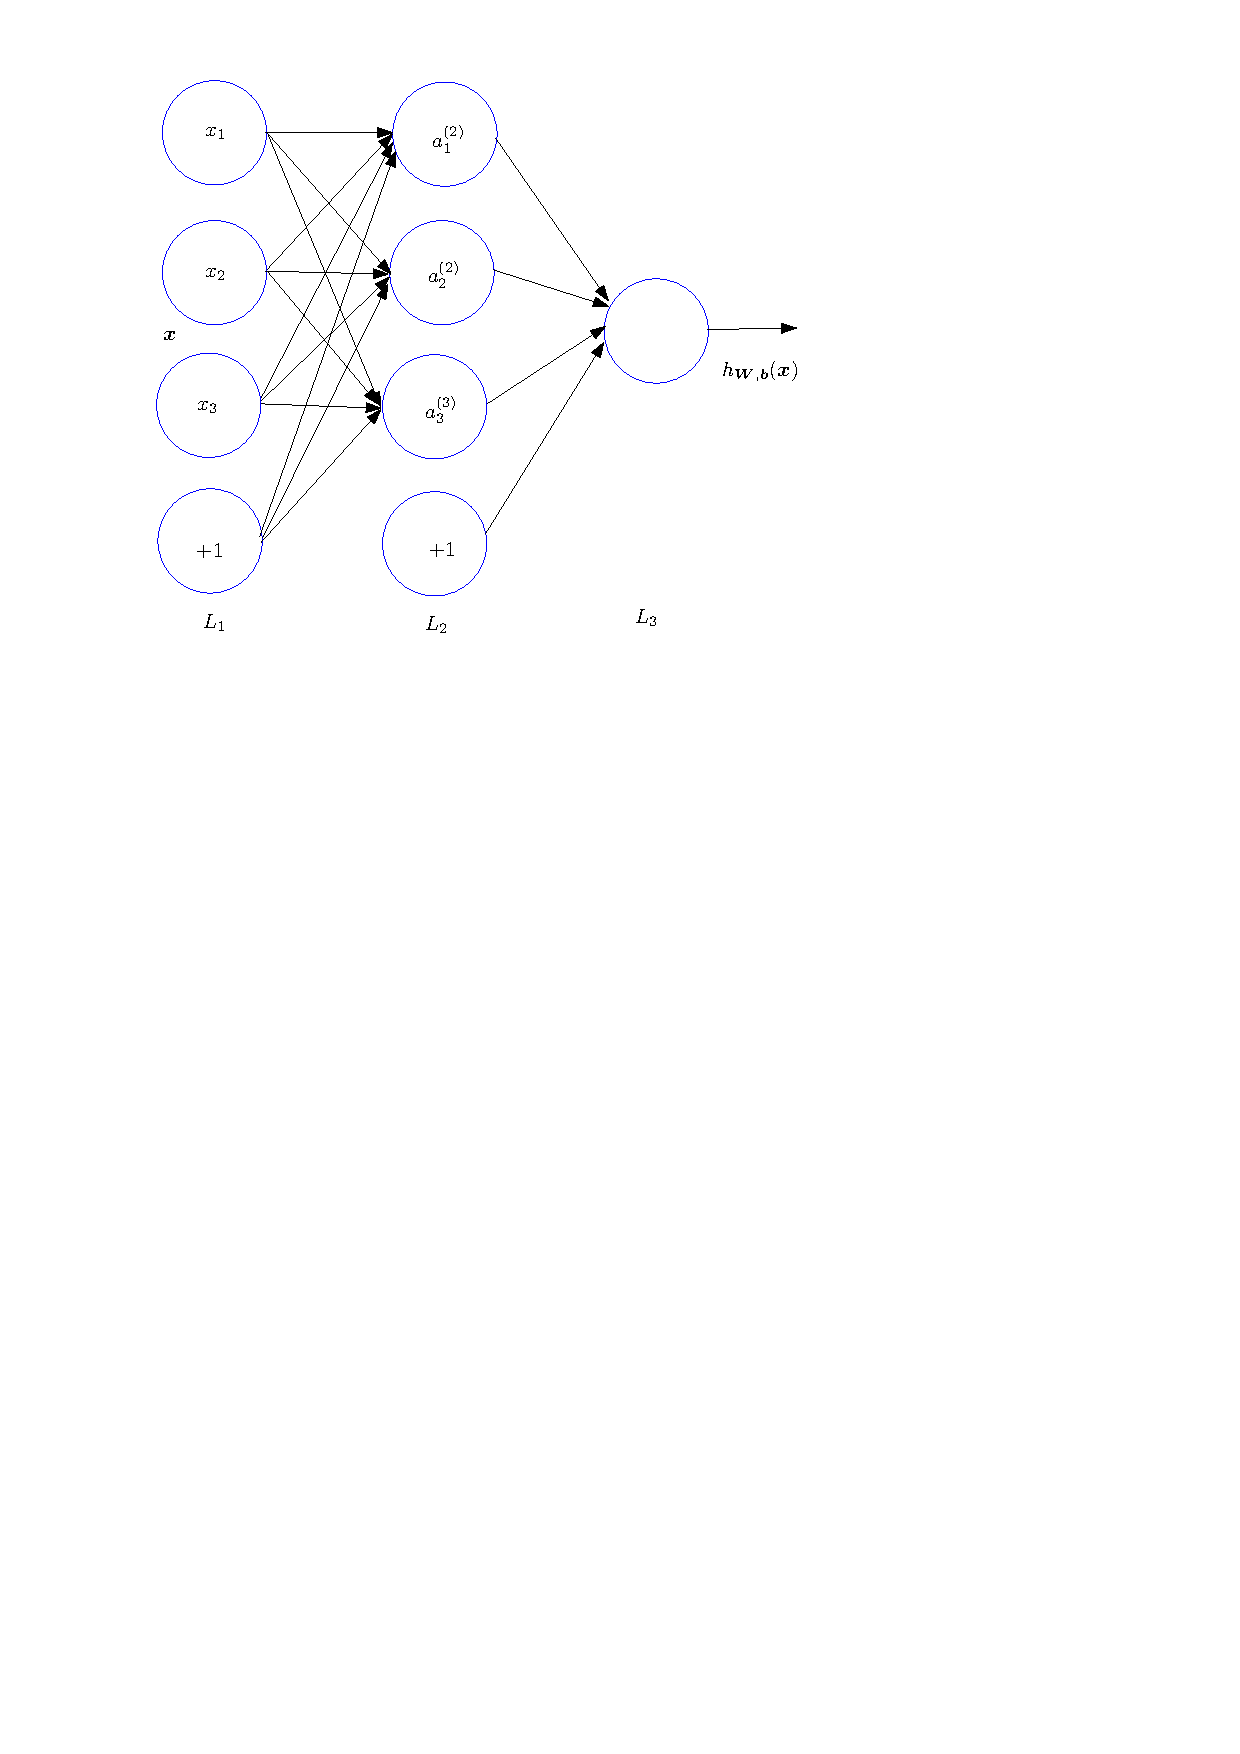
\includegraphics[width = 0.60 \textwidth]{notation.pdf}
  \caption{模型示意图}
  \label{notation}
\end{figure}

每一个圆圈称为一个单元(节点), 次序从上到下. 其中标上“+1”的圆圈称为偏置节点, 也就是截距项.神经网络最左边的一层叫做输入层, 最右的一层叫做输出层(本图中, 输出层只有一个节点, 可以描述二分类, 如果有多个节点可以描述多分类, 如手写数字识别). 中间所有节点组成的层叫做隐藏层, 因为我们不能在训练样本集中观测到它们的值. 同时可以看到, 以上神经网络的例子中有3个输入单元(偏置单元不计在内), 3个隐藏单元及一个输出单元. 接下来符号“轰炸”而来, 做好准备.

我们用$L$表示网络的层数, 本图中$L = 3$, 我们将第$l$层记为$L_{l}$, 于是输入层是$L_{1}$, 本图中输出层是$L_{3}$, 设第$l$层神经元的个数为$s_{l}$. 用$a_{i}^{(l)}$表示第$l$层第$i$单元的激活值(当$l = 1$时, $a_{i}^{(l)} = x_{i}$), 同时把整个第$l$层的激活值并成列向量$\bm{a}^{(l)}$来表示.

我们知道$a_{i}^{(l)}(l \geqslant 2)$是由前一层算出来的, 设$b_{i}^{(l)}$表示(第$l$层到)第$l + 1$层第$i$单元的偏置项(这样可让$l$从1开始, 否则如果用$b_{i}^{(l)}$表示第$l$层第$i$单元的偏置项, 那么$l$就应该从2开始, 这样当然也可以处理, 不过脚标不从1开始可能有些别扭, 下面的$w_{ij}^{(l)}$同理), 用$w_{ij}^{(l)}$表示第$l$层第$j$单元到第$l + 1$层第$i$单元之间的连接参数(也就是连接线上的权重, 格外注意此处的标号顺序), 用$z_{i}^{(l)}$表示第$l$层第$i$单元的状态, 可以这样理解: 要想计算第$l$层第$i$单元的活性值$a_{i}^{(l)}(l \geqslant 2)$, 需要利用偏置$b_{i}^{(l - 1)}$和权重$w_{ij}^{(l - 1)}$, 反正上标中的$l$表示的是第$l$层, 下标中的$i$是该层的第$i$单元, 而下标中的$j$一般是求和指标, 对该层中的所有神经元求和, 在本例中, 也即为
\begin{align*}
a_{1}^{(2)} & = f(z_{1}^{(2)}) = f(w_{11}^{(1)} x_1 + w_{12}^{(1)} x_2 + w_{13}^{(1)} x_3 + b_{1}^{(1)}) \\ 
a_{2}^{(2)} & = f(z_{2}^{(2)}) = f(w_{21}^{(1)} x_1 + w_{22}^{(1)} x_2 + w_{23}^{(1)} x_3 + b_{2}^{(1)}) \\ 
a_{3}^{(2)} & = f(z_{3}^{(2)}) = f(w_{31}^{(1)} x_1 + w_{32}^{(1)} x_2 + w_{33}^{(1)} x_3 + b_{3}^{(1)}) \\ 
a_{1}^{(3)} & = f(z_{1}^{(3)}) = f(w_{11}^{(2)} a_{1}^{(2)} + w_{12}^{(2)} a_{2}^{(2)} + w_{13}^{(2)} a_{3}^{(2)} + b_{1}^{(2)})
\end{align*}

为了书写的方便, 我们也把第$l$层的状态值并成列向量$\bm{z}^{(l)}$来表示, 同时把权重系数也并起来, 即用$W^{(l)}$表示第$l$层到第$l + 1$层的权重矩阵, $W^{(l)}$的$(i, j)$元就是$w_{ij}^{(l)}$, 把整个神经网络的所有权重矩阵统记为$\bm{W}$, 而所有的偏置向量统记为$\bm{b}$, 同时扩展函数表示符号的定义, 即编程中的向量化(一个函数作用到一个向量或者矩阵上, 相当于作用到它每个分量上), 这样就有
\begin{align*}
\bm{z}^{(2)} & = W^{(1)} \bm{x} + \bm{b}^{(2)} \\ 
\bm{a}^{(2)} & = f(\bm{z}^{(2)}) \\ 
\bm{z^{(3)}} & = W^{(2)} \bm{a}^{(2)} + \bm{b}^{(3)} \\ 
h_{\bm{W, b}} (\bm{x}) & = \bm{a}^{(3)} = f(\bm{z}^{(3)}) 
\end{align*}

当然, 在本例中最后的$\bm{z}^{(3)}$和$\bm{a}^{(3)}$实际上只有一个分量, 而权重矩阵$W^{(1)} \in \mathbb{R}^{3 \times 3}, W^{(2)} \in \mathbb{R}^{1 \times 3}$.

我们将上面的步骤称为前向传播. 回想一下, 之前用$\bm{a}^{(1)} = \bm{x}$表示输入层的激活值, 那么给定第$l$层的激活值$\bm{a}^{(l)}$后, 第$l + 1$层的激活值$\bm{a}^{(l + 1)}$就可以按照下面步骤计算得到:
\begin{align*}
\bm{z}^{(l + 1)} & = W^{(l)} \bm{a}^{(l)} + \bm{b}^{(l)} \\ 
\bm{a}^{(l + 1)} & = f(\bm{z}^{(l + 1)})
\end{align*}

也就是说前馈神经网络是通过信息的逐层传递, 得到网络最后的输出$\bm{a}^{(n_l)}$.
\begin{equation*}
\bm{x} = \bm{a}^{(1)} \rightarrow \bm{z}^{(2)} \rightarrow \bm{a}^{(2)} \rightarrow \bm{z}^{(3)} \rightarrow \cdots \rightarrow \bm{a}^{(L - 1)} \rightarrow \bm{z}^{(L)} \rightarrow \bm{a}^{(L)} = \bm{y}
\end{equation*}

这就是一个完整的前向神经网络模型, 我们的目的便是通过已有的$m$个训练样本$(\bm{x}^{(i)}, \bm{y}^{(i)}), i = 1, 2, \cdots, m$, 来求出最优的模型参数$\bm{W}$和$\bm{b}$, 使得模型能够很好的拟合样本数据, 并能用来进行很好的预测.


\subsection{参数估计}
那么我们如何求得模型的最优参数呢?

前面已多次提到, 机器学习的框架是构造损失函数或者代价函数来极小化得到参数估计, 这里我们用最小二乘的思想, 对于单个样本$(\bm{x}, \bm{y})$, 我们构造其代价函数为
\begin{equation*}
J(\bm{W}, \bm{b}; \bm{x}, \bm{y}) = \frac{1}{2} ||h_{\bm{W}, \bm{b}}(\bm{x}) - \bm{y}||^2
\end{equation*}

给定一个包含$m$个样本的数据集, 我们可以定义整体代价函数为
\begin{align*}
J(\bm{W},\bm{b}) & = \left[ \frac{1}{m} \sum_{i=1}^{m} J(\bm{W},\bm{b}; \bm{x}^{(i)},\bm{y}^{(i)}) \right] + \frac{\lambda}{2m} \sum_{l=1}^{L-1} \sum_{i=1}^{s_{l+1}} \sum_{j=1}^{s_{l}} (w_{ij}^{(l)})^2 \\
& = \left[ \frac{1}{m} \sum_{i=1}^{m} \left( \frac{1}{2} ||h_{\bm{W},\bm{b}}(\bm{x}^{(i)}) - \bm{y}^{(i)}||^2 \right) \right] + \frac{\lambda}{2m} \sum_{l=1}^{L-1} \sum_{i=1}^{s_{l+1}} \sum_{j=1}^{s_{l}} (w_{ij}^{(l)})^2
\end{align*}

我们在这里直接进行了正则化, 即加入了对参数$\bm{W}$的惩罚, 防止过拟合. 注意一下记号: $J(\bm{W},\bm{b}; \bm{x},\bm{y})$是针对单个样本的代价函数, $J(\bm{W},\bm{b})$是整体样本的代价函数, 它包含正则化项.

我们的目标是针对参数$\bm{W}$和$\bm{b}$极小化代价函数$J(\bm{W},\bm{b})$. 这里, 我们还是采用最常用的梯度下降法. 即先将每一个参数$w_{ij}^{(l)}$和$b_{i}^{(l)}$初始化一个很小的、接近于$0$的随机值(比如使用正态分布$\mathcal{N}(0, \varepsilon^2)$生成的随机值, 其中$\varepsilon$可设置为$0.01$), 之后对目标函数使用梯度下降法. 因为这里的$J(\bm{W}, \bm{b})$是一个非凸函数, 梯度下降法很可能会收敛到一个局部最优解, 但在实际应用中, 梯度下降法常常能得到令人满意的结果. 需要再次强调一点, 就是这里一定要将参数随机初始化, 而不是如通常一般全置为$0$, 因为如果所有参数都用相同的值作为初始值, 那么所有隐藏单元最终会得到与输入值有关的、相同的函数(也就是说, 对于所有$i$, $w_{ij}^{(l)}$都会取相同的值, 那么对于任何输入$\bm{x}$, 都会有$\bm{a}^{(1)} = \bm{a}^{(2)} = \bm{a}^{(3)} = \cdots$). 随机初始化的目的是使对称失效.

梯度下降法的更新公式为
\begin{align*}
w_{ij}^{(l)} & := w_{ij}^{(l)} - \alpha \frac{\partial}{\partial w_{ij}^{(l)}} J(\bm{W}, \bm{b}) \\ 
b_{i}^{(l)} & := b_{i}^{(l)} - \alpha \frac{\partial}{\partial b_{i}^{(l)}} J(\bm{W}, \bm{b})
\end{align*}

这里面好像偏导数很难计算, 因为以前比如线性回归、Logistic回归的目标函数都很清楚, 但这里$J(\bm{W},\bm{b})$的具体表达式根本不知道, 神经网络是个多层模型, 它嵌套了多个复合函数, 似乎让我们无从下手, 不过, 我们还是有办法的, 那就是反向传播算法(Backpropagation Algorithm), 所以大多数文献里的神经网络都是 BP 神经网络, 这里“BP”指的就是反向传播算法.

反向传播算法的推导过程看似很繁, 但其实不难, 既然是嵌套了多个复合函数, 那求偏导过程自然主要利用了复合函数求导的链导法则, 仅此而已, 下面我们就来推导一下反向传播算法.


\subsection{反向传播算法}
我们先来讲一下对于单个样本$(\bm{x},\bm{y})$, 如何用反向传播算法来计算代价函数$J(\bm{W},\bm{b}; \bm{x},\bm{y})$对参数$w_{ij}^{(l)}$和$b_{i}^{(l)}$的偏导数. 一旦求出该偏导数, 就可以推导出整体代价函数$J(\bm{W},\bm{b})$的偏导数了.
\begin{align*}
\frac{\partial}{\partial w_{ij}^{(l)}} J(\bm{W},\bm{b}) & = \left[\ \frac{1}{m} \sum_{i=1}^{m} \frac{\partial}{\partial w_{ij}^{(l)}} J(\bm{W},\bm{b}; \bm{x}^{(i)},\bm{y}^{(i)}) \right] + \frac{\lambda}{m} w_{ij}^{(l)} \\ 
\frac{\partial}{\partial b_{i}^{(l)}} J(\bm{W},\bm{b}) & = \frac{1}{m} \sum_{i=1}^{m} \frac{\partial}{\partial b_{i}^{(l)}} J(\bm{W},\bm{b}; \bm{x}^{(i)},\bm{y}^{(i)})
\end{align*}

反向传播算法的思路如下: 给定一个样本$(\bm{x}, \bm{y})$, 我们首先进行“前向传导”运算, 由于参数已经初始化赋值, 因此可以计算出网络中所有的激活值, 包括$h_{\bm{W},\bm{b}}$的输出值. 之后, 就要按照梯度下降法更新参数了, 也就是需要求出偏导数. 怎么做呢? 我们是通过一个中间量来计算的. 针对第$l$层的每一个节点$i$, 我们定义一个量$\delta_{i}^{(l)}$, 称为“残差”, 其值定义为样本代价函数$J(\bm{W},\bm{b}; \bm{x},\bm{y})$对该节点的活性值$z_{i}^{(l)}$的偏导数, 该残差表明了该节点对最终输出值的残差产生了多少影响.

我们先来看如何计算残差这个量, 再讲如何利用残差计算我们需要的偏导数. 残差的计算方法如下:
\begin{enumerate}[(1)]
\item 进行前馈传导计算, 根据样本值和初始参数值, 得到$L_{2}, L_{3}, \cdots$直到输出层的激活值.

\item 计算第$L$层, 也就是输出层的残差, 对于第$L$层的每个输出单元$i$, 根据以下公式计算残差:
\begin{equation*}
\delta_{i}^{(L)} = -(y_{i} - a_{i}^{(L)}) \cdot f'(z_{i}^{(L)})
\end{equation*}

事实上, 根据定义, 用链导法则计算可得
\begin{align*}
\delta_{i}^{(L)} & = \frac{\partial}{\partial z_{i}^{(L)}} J(\bm{W},\bm{b}; \bm{x},\bm{y}) = \frac{\partial}{\partial z_{i}^{(L)}} \frac{1}{2} ||\bm{y} - h_{\bm{W},\bm{b}}(\bm{x})||^2 \\ 
& = \frac{\partial}{\partial z_{i}^{(L)}} \frac{1}{2} \sum_{j=1}^{s_L}(y_{j} - a_{j}^{(L)})^2 = \frac{\partial}{\partial z_{i}^{(L)}} \frac{1}{2} \sum_{j=1}^{s_L} (y_{j} - f(z_{j}^{(L)}))^2 \\ 
& = -(y_{i} - f(z_{i}^{(L)})) \cdot f'(z_{i}^{(L)}) = -(y_{i} - a_{i}^{(L)}) \cdot f'(z_{i}^{(L)})
\end{align*}


\item 依次计算$l = L-1, L-2, L-3, \cdots, 2$的各个层, 第$l$层的第$i$个节点的残差计算公式如下:
\begin{equation*}
\delta_{i}^{(l)} = \left( \sum_{j=1}^{s_{l+1}} w_{ji}^{(l)} \delta_{j}^{(l+1)} \right) f'(z_{i}^{(l)})
\end{equation*}

比如先计算第$L - 1$层的残差, 根据定义, 用链导法则可得
\begin{align*}
\delta_{i}^{(L-1)} & = \frac{\partial}{\partial z_{i}^{(L-1)}} J(\bm{W},\bm{b};\bm{x},\bm{y}) = \frac{\partial}{\partial z_{i}^{(L-1)}} \frac{1}{2} ||\bm{y} - h_{\bm{W},\bm{b}}(\bm{x})||^2 = \frac{\partial}{\partial z_{i}^{(L-1)}} \frac{1}{2} \sum_{j=1}^{s_L} (y_{j} - a_{j}^{(L)})^2 \\ 
& = \frac{1}{2} \sum_{j=1}^{s_L} \frac{\partial}{\partial z_{i}^{(L-1)}} (y_{j} - a_{j}^{(L)})^2 = \frac{1}{2} \sum_{j=1}^{s_L} \frac{\partial}{\partial z_{i}^{(L-1)}} (y_{j} - f(z_{j}^{(L)}))^2 \\ 
& = \sum_{j=1}^{s_L} -(y_{j} - f(z_{j}^{(L)})) \cdot \frac{\partial}{\partial z_{i}^{(L-1)}} f(z_{j}^{(L)}) = \sum_{j=1}^{s_L} -(y_{j} - f(z_{j}^{(L)})) \cdot f'(z_{j}^{(L)}) \cdot \frac{\partial z_{j}^{(L)}}{\partial z_{i}^{(L-1)}} \\ 
& = \sum_{j=1}^{s_L} \delta_{j}^{(L)} \cdot \frac{\partial z_{j}^{(L)}}{\partial z_{i}^{(L-1)}} = \sum_{j=1}^{s_L} \left( \delta_{j}^{(L)} \cdot \frac{\partial}{\partial z_{i}^{(L-1)}} \sum_{k=1}^{s_{L-1}} f(z_{k}^{(L-1)}) \cdot w_{jk}^{(L-1)} \right) \\ 
& = \sum_{j=1}^{s_L} \delta_{j}^{(L)} \cdot w_{ji}^{(L-1)} \cdot f'(z_{i}^{(L-1)}) = \left( \sum_{j=1}^{s_L} w_{ji}^{(L-1)} \delta_{j}^{(L)} \right) f'(z_{i})^{(L-1)}
\end{align*}

同理, 若已知第$l + 1$层的残差, 要计算第$l$层的残差, 将上式中的$L - 1$与$L$的关系替换为$l$与$l + 1$的关系(暂时没有想明白为什么可以替换), 可得
\begin{equation*}
\delta_{i}^{(l)} = \left( \sum_{j=1}^{s_{l+1}} w_{ji}^{(l)} \delta_{j}^{(l+1)} \right) f'(z_{i}^{(l)})
\end{equation*}

以上逐次从后向前求导的过程即为“反向传导”的本意所在.
\end{enumerate}

有了残差, 就可以计算我们需要的偏导数了, 公式如下:
\begin{align*}
\frac{\partial}{\partial w_{ij}^{(l)}} J(\bm{W},\bm{b};\bm{x},\bm{y}) & = a_{j}^{(l)} \delta_{i}^{(l+1)} \\ 
\frac{\partial}{\partial b_{i}^{(l)}} J(\bm{W},\bm{b};\bm{x},\bm{y}) & = \delta_{i}^{(l+1)}
\end{align*}

事实上, 引入中间变量$z_{i}^{(l+1)}$, 有
\begin{align*}
\frac{\partial}{\partial w_{ij}^{(l)}} J(\bm{W},\bm{b};\bm{x},\bm{y}) & = \frac{\partial J(\bm{W},\bm{b};\bm{x},\bm{y})}{\partial z_{i}^{(l+1)}} \cdot \frac{\partial z_{i}^{(l+1)}}{\partial w_{ij}^{(l)}} \\ 
& = \delta_{i}^{(l+1)} \cdot \frac{\partial z_{i}^{(l+1)}}{\partial w_{ij}^{(l)}}
\end{align*}

至于第二项, 我们知道
\begin{align*}
\bm{z}^{(l+1)} & = W^{(l)} \bm{a}^{(l)} + \bm{b}^{(l)} \\ 
z_{i}^{(l+1)} & = w_{i1}^{(l)} a_{1}^{(l)} + w_{i2}^{(l)} a_{2}^{(l)} + \cdots + w_{is_{l}}^{(l)} a_{s_l}^{(l)} + b_{i}^{(l)}
\end{align*}

因此有
\begin{equation*}
\frac{\partial z_{i}^{(l+1)}}{\partial w_{ij}^{(l)}} = a_{j}^{(l)}
\end{equation*}

于是可得
\begin{equation*}
\frac{\partial}{\partial w_{ij}^{(l)}} J(\bm{W},\bm{b};\bm{x},\bm{y}) = \delta_{i}^{(l+1)} \cdot \frac{\partial z_{i}^{(l+1)}}{\partial w_{ij}^{(l)}} =  \delta_{i}^{(l+1)} a_{j}^{(l)}
\end{equation*}

同理可得
\begin{equation*}
\frac{\partial}{\partial b_{i}^{(l)}} J(\bm{W},\bm{b};\bm{x},\bm{y}) = \frac{\partial J(\bm{W},\bm{b};\bm{x},\bm{y})}{\partial z_{i}^{(l+1)}} \cdot \frac{\partial z_{i}^{(l+1)}}{\partial b_{i}^{(l)}} = \delta_{i}^{(l+1)} \cdot 1 = \delta_{i}^{(l+1)}
\end{equation*}

至此, 如何计算偏导数已经讲完了.

最后, 我们将公式向量化, 采用我们矩阵分析里讲的 Hardmard 乘积符号$\circ$, 即对应元素相乘(在 Matlab 中用“ .* ”表示), 那么反向传播算法可表示为以下几个步骤:
\begin{enumerate}[(1)]
\item 进行前馈传导计算, 利用前向传导公式, 得到$L_{2}, L_{3}, \cdots$直到输出层的激活值.

\item 对输出层(第$L$层), 计算
\begin{equation*}
\bm{\delta}^{(L)} = -(\bm{y} - \bm{a}^{(L)}) \circ f'(\bm{z}^{(L)})
\end{equation*}

\item 对于$l = L-1, L-2, L-3, \cdots, 2$的各层, 计算
\begin{equation*}
\bm{\delta}^{(l)} = ((W^{(l)})^{T} \bm{\delta}^{(l + 1)}) \circ f'(\bm{z}^{(l)})
\end{equation*}

\item 计算最终需要的偏导数值:
\begin{align*}
\nabla_{W^{(l)}} J(\bm{W},\bm{b};\bm{x},\bm{y}) & = \bm{\delta}^{(l+1)} (\bm{a}^{(l)})^{T} \\ 
\nabla_{\bm{b}^{(l)}} J(\bm{W},\bm{b}; \bm{x},\bm{y}) & = \bm{\delta}^{(l+1)}
\end{align*}

\end{enumerate}

编程时应注意, 计算$f'(\bm{z})$时, 由于我们的激活函数选的是 sigmoid 函数,因此根据 sigmoid 函数的性质有$f'(z_{i}^{(l)}) = a_{i}^{(l)} (1 - a_{i}^{(l)})$.

以上便是对单个样本$(\bm{x},\bm{y})$如何计算偏导数的过程, 最后, 假设有$m$个样本$(\bm{x}^{(i)}, \bm{y}^{(i)})$, 我们对梯度下降法做个总结, 过程如下:
\begin{enumerate}[(1)]
\item 对于所有$l$, 令$\Delta W^{(l)} := 0, \Delta \bm{b}^{(l)} = 0$(设置为全零矩阵和全零向量)

\item  for i = 1 to m
\begin{itemize}
\item 使用反向传播算法计算$\nabla_{W^{(l)}} J(\bm{W},\bm{b};\bm{x},\bm{y})$ 和 $\nabla_{\bm{b}^{(l)}} J(\bm{W},\bm{b}; \bm{x},\bm{y})$

\item 令 $\Delta W^{(l)} := \Delta W^{(l)} + \nabla_{W^{(l)}} J(\bm{W},\bm{b}; \bm{x},\bm{y})$

\item 令 $\Delta \bm{b}^{(l)} := \Delta \bm{b}^{(l)} + \nabla_{\bm{b}^{(l)}} J(\bm{W},\bm{b}; \bm{x},\bm{y})$
\end{itemize}

\item 更新参数:
\begin{align*}
W^{(l)} & := W^{(l)} - \alpha \left[ \left( \frac{1}{m} \Delta W^{(l)} \right) + \frac{\lambda}{m} W^{(l)} \right] \\ 
\bm{b}^{(l)} & := \bm{b}^{(l)} - \alpha \left[ \frac{1}{m} \Delta \bm{b}^{(l)} \right]
\end{align*}


\end{enumerate}

以上式中的$\Delta W^{l}$和$\Delta \bm{b}^{(l)}$并不表示 Laplace 算子,而只是一个增量表示, 用来累加总的梯度而已.

完整的梯度下降法终于讲完了, 反复迭代便可以求解我们的神经网络了.


\section{关于前向神经网络的补充}
\subsection{反向传播算法的推导}
反向传播算法是计算偏导数的关键, 也是梯度下降法的关键, 上面的推导过程来自 \url{http://deeplearning.stanford.edu/wiki/index.php/%E5%8F%8D%E5%90%91%E4%BC%A0%E5%AF%BC%E7%AE%97%E6%B3%95}, 但是我对那个直接替换的一步有些怀疑, 因此参考了其他资料, 在此写一下其它推导方法.

不过, 在此之前, 我们再说明一下模型所用符号, 几乎都同前面一样, 只有$w_{ij}^{(l)}$和$b_{i}^{(l)}$, 这在前面也提到了, 不管怎么规定都有“违和”之处, 这里, 将$b_{i}^{(l)}$表示为第$l$层第$i$单元的偏置项, 同理$w_{ij}^{(l)}$表示第$l - 1$层第$j$单元到第$l$层第$i$单元的权重, 前面说过, 这样更为自然, 但此时$l$就从$2$开始了. 相应的, $W^{(l)}$表示第$l - 1$层到第$l$层的权重矩阵($l$从$2$开始), 有$W^{(l)} \in \mathbb{R}^{s_l \times s_{l-1}}$, $\bm{b}^{(l)}$表示(第$l-1$层到)第$l$层的偏置, 其它记号不变.

如此一来, 模型的前向传递过程可以表示为
\begin{align*}
\bm{z}^{(l)} & = W^{(l)} \cdot \bm{a}^{(l-1)} + \bm{b}^{(l)} \\ 
\bm{a}^{(l)} & = f(\bm{z}^{(l)})
\end{align*}

也可以合并写为
\begin{align*}
\bm{z}^{(l-1)} & = W^{(l)} \cdot f(\bm{z}^{(l-1)}) + \bm{b}^{(l)} \\
\bm{a}^{(l)} & = f(\bm{z}^{(l)}) = f(W^{(l)} \bm{a}^{(l-1)} + \bm{b}^{(l)})
\end{align*}

写成分量形式
\begin{equation*}
a_{i}^{(l)} = f(z_{i}^{(l)}) = f(\sum_{j=1}^{s_{l-1}} w_{ij}^{(l)} a_{j}^{(l-1)} + b_{j}^{(l)})
\end{equation*}

下面来推导反向传播算法, 主要是“残差”的计算.

对于第$L$层也就是输出层, 有
\begin{align*}
\delta_{i}^{(L)} & = \frac{\partial J(\bm{W},\bm{b};\bm{x},\bm{y})}{\partial z_{i}^{(L)}} = \sum_{j=1}^{s_L} \frac{\partial J(\bm{W},\bm{b};\bm{x},\bm{y})}{\partial a_{j}^{(L)}} \cdot \frac{\partial a_{j}^{(L)}}{\partial z_{i}^{(L)}} \\ 
& = \frac{\partial J(\bm{W},\bm{b};\bm{x},\bm{y})}{\partial a_{i}^{(L)}} \cdot \frac{\partial a_{i}^{(L)}}{\partial z_{i}^{(L)}} \\ 
& = \frac{\partial}{\partial a_{i}^{(L)}} \frac{1}{2} \sum_{j=1}^{s_L} (y_{j} - a_{j}^{(L)})^2 \cdot f'(z_{i}^{(L)}) \\ 
& = (a_{i}^{(L)} - y_{i}) \cdot f'(z_{i}^{(L)})
\end{align*}

接下来看如何由第$l + 1$层计算第$l$层, 还是运用链导法则, 可得
\begin{align*}
\delta_{i}^{(l)} & = \frac{\partial J(\bm{W},\bm{b};\bm{x},\bm{y})}{\partial z_{i}^{(l)}} \\ 
& = \sum_{j=1}^{s_{l+1}} \frac{\partial J(\bm{W},\bm{b};\bm{x},\bm{y})}{\partial z_{j}^{(l+1)}} \cdot \frac{\partial z_{j}^{(l+1)}}{\partial z_{i}^{(l)}} \\ 
& = \sum_{j=1}^{s_{l+1}}  \frac{\partial z_{j}^{(l+1)}}{\partial z_{i}^{(l)}} \delta_{j}^{(l+1)}
\end{align*}

注意到
\begin{equation*}
z_{j}^{(l+1)} = \sum_{i=1}^{s_l} w_{ji}^{(l+1)} a_{i}^{(l)} + b_{j}^{(l+1)} = \sum_{i=1}^{s_l} w_{ji}^{(l+1)} f(z_{i}^{(l)}) + b_{j}^{(l+1)}
\end{equation*}

求导可得
\begin{equation*}
\frac{\partial z_{j}^{(l+1)}}{\partial z_{i}^{(l)}} = w_{ji}^{(l+1)} f'(z_{i}^{(l)})
\end{equation*}

于是可得
\begin{equation*}
\delta_{i}^{(l)} = \left( \sum_{j=1}^{s_{l+1}} w_{ji}^{(l+1)} \delta_{j}^{(l+1)} \right) f'(z_{i}^{(l)})
\end{equation*}

这样我们就完成了证明, 该证明可见\url{http://neuralnetworksanddeeplearning.com/chap2.html}, 这里注意$w_{ji}^{(l + 1)}$的上脚标是$l + 1$, 而不是上面的$l$, 因为定义$w_{ij}^{(l)}$时有所不同.

当然, 熟练的话, 可以以向量的形式求导, 如下:
\begin{align*}
\bm{\delta}^{(l)} & = \frac{\partial J(\bm{W},\bm{b};\bm{x},\bm{y})}{\partial \bm{z}^{(l)}} \\ 
& = \frac{\partial \bm{a}^{(l)}}{\partial \bm{z}^{(l)}} \cdot \p{}{\bm{z}^{(l+1)}}{\bm{a}^{(l)}} \cdot \p{}{J(\bm{W},\bm{b};\bm{x},\bm{y})}{\bm{z}^{(l+1)}} \\ 
& = \mathrm{diag}(f'(\bm{z}^{(l)})) \cdot (W^{(l+1)})^{T} \cdot \bm{\delta}^{(l+1)} \\ 
& = f'(\bm{z}^{(l)}) \circ \left( (W^{(l+1)})^{T} \cdot \bm{\delta}^{(l+1)} \right)
\end{align*}

其中, 因为$\bm{z}^{(l+1)} = W^{(l+1)} \cdot \bm{a}^{(l)} + \bm{b}^{(l)}$, 所以
\begin{equation*}
\p{}{\bm{z}^{(l+1)}}{\bm{a}^{(l)}} = (W^{(l+1)})^{T}
\end{equation*}

又因为$\bm{a}^{(l)} = f(\bm{z}^{(l)})$, 而我们已使函数向量化, 因此有
\begin{equation*}
\p{}{\bm{a}^{(l)}}{\bm{z}^{(l)}} = \p{}{f(\bm{z}^{(l)})}{\bm{z}^{(l)}} = \mathrm{diag} (f'(\bm{z}^{(l)}))
\end{equation*}

可以看出, 反向传播算法的含义是: 第$l$层的一个神经元的误差项是所有与该神经元相连的第$l + 1$层的神经元的误差项的权重和, 然后再乘上该神经元激活函数的梯度.


\subsection{关于激活函数的选择}
以上我们主要是采用 sigmoid 激活函数进行的叙述和推导, 不过前面已经提到, 激活函数有很多选择, 比如还可以选为 tanh 函数, 此外, 还有一个很重要的激活函数, 称为 rectified linear neuron 或 rectified linear unit, 简称为 ReLU, 其形式为
\begin{equation*}
f(x) = \max (0, z), \quad \textrm{即} \quad a = \max(0, \bm{w}^{T} \bm{x} + b)
\end{equation*}

不管采用哪种激活函数, 相应的反向传播算法都比较类似, 至于具体问题中该如何选择激活函数, 这是一个复杂的问题, 相关讨论可参考: \url{http://neuralnetworksanddeeplearning.com/chap3.html#other_models_of_artificial_neuron}.


\subsection{梯度消失问题}
误差反向传播的迭代公式为
\begin{equation*}
\bm{\delta}^{(l)} = f'(\bm{z}^{(l)}) \circ \left( (W^{(l+1)})^{T} \cdot \bm{\delta}^{(l+1)} \right)
\end{equation*}

其中需要用到激活函数$f(\cdot)$的导数, 即当误差从输出层反向传播时,在每一层都要乘以该层的激活函数的导数, 当我们使用 sigmoid 函数或者 tanh 函数时, 其导数为
\begin{align*}
\sigma'(x) & = \sigma(x) (1 - \sigma(x)) \in [0, 0.25] \\ 
\tanh'(x) & = 1 - (\tanh(x))^2 \in [0, 1] \\ 
\end{align*}

即此两者激活函数的值域都小于 1, 这样误差经过每一层传递都会不断衰减. 当网络层数很深时, 梯度就会不停的衰减甚至消失, 使得整个网络很难训练.这就是所谓的梯度消失问题(Vanishing Gradient Problem), 也叫梯度弥散.

减轻梯度消失问题的一个方法便是使用上面的 ReLU 激活函数, 其导数为 1, 误差可以很好的传播, 训练速度也因此可以得到提高.


\subsection{关于损失函数的确定}
上面我们构造的代价函数称为平方误差损失函数(Squared Error Loss Function), 不过实际上还有另外一个流行的损失函数, 与 Softmax 回归的损失函数是类似的, 称为交叉熵(Cross Entropy), 如下
\begin{equation*}
J(\Theta) = - \sum_{i=1}^{m} \sum_{k=1}^{K} \mathbb{I} \{y^{(i)} = k \} \ln \frac{\exp (\bm{\theta}^{(k) \mathrm{T}} h_{\Theta}(\bm{x}^{(i)}))} {\sum_{j=1}^{K} \exp (\bm{\theta}^{(j) \mathrm{T}} h_{\Theta}(\bm{x}^{(i)}))}
\end{equation*}

注意这里用$\Theta$表示所有的参数, 用$y = k$表示样本属于第$k$类(而不是向量的方式), 上式来自于 \url{http://ufldl.stanford.edu/tutorial/supervised/ExerciseSupervisedNeuralNetwork/}, 是 Andrew Ng 的 Ufldl 的一篇文章. 容易看出这与 Softmax 的代价函数是极为相似的. 此时计算梯度的方法还是反向传播算法.

Andrew Ng 在 Coursera 的公开课中(\url{https://class.coursera.org/ml-005/lecture})中也讲了前向神经网络模型, 在那里定义损失函数时, 是直接仿照 Logistic 回归的损失函数的, 如下式
\begin{equation*}
J(\Theta) = - \frac{1}{m} \left[ \sum_{i=1}^{m} \sum_{k=1}^{K} y_{k}^{(i)} \ln (h_{\Theta}(\bm{x}^{(i)}))_{k} + (1 - y_{k}^{(i)}) \ln (1 - (h_{\Theta}(\bm{x}^{(i)}))_{k}) \right]
\end{equation*}

这里对应的类别是用向量$\bm{y}$表示的, 对应的梯度计算也是反向传播算法, 具体可见他课程的 Lecture 9.

实际上, R 语言的 neuralnet 包中的 neuralnet 函数就提供了参数, 可以选择代价函数的方式: 平方误差或者交叉熵. 当然, 该函数计算梯度时可以改换参数不使用反向传播算法, 具体细节这里就不提了.





\section{贝叶斯方法}









\section{总结}
\begin{enumerate}[(1)]
\item Andrew Ng 的深度学习入门, 可见 \url{http://deeplearning.stanford.edu/wiki/index.php/UFLDL_Tutorial}, 中文翻译网页是 \url{http://deeplearning.stanford.edu/wiki/index.php/UFLDL%E6%95%99%E7%A8%8B}, 讲的还行, 主要是符号与之前的比较一致, 主要参考了前两节, 后面的内容以后可以细看

\item Michael Nielsen 的《Neural Networks and Deep Learning》, 一本在线书, 讲的相当不错, 可见 \url{http://neuralnetworksanddeeplearning.com/index.html}, 还有 Python 实现的代码, 以后有时间要看后面的部分.

\item 邱锡鹏的《神经网络与深度学习讲义》, 推导的不错.

\item 博客: \url{http://www.di.fc.ul.pt/~jpn/r/neuralnets/neuralnets.html}, 一个用 R 计算神经网络的小例子, 还不错, 应该是用 RMarkdown 写的.

\item 博客: \url{https://people.phys.ethz.ch/~evertv/weekendprojects/NeuralNet-MNIST.html}, 是用 ipython notebook 写的, 用 Python 实现了 BP 神经网络.

\item 博客: \url{http://www.wildml.com/2015/09/implementing-a-neural-network-from-scratch/}, 也是用 Python 实现了 BP 神经网络, 也有相应的 ipython notebook 源文件, 并且画出了决策边界(决策边界大全: \url{http://www.subsubroutine.com/sub-subroutine/2016/2/15/understanding-machine-learning-techniques-by-the-decision-boundaries-they-are-capable-of}). 其实用 Python 实现的很多, 比如还有 \url{https://triangleinequality.wordpress.com/2014/03/31/neural-networks-part-2/}
\end{enumerate}



\newpage

\section*{附录}








\end{document}